\documentclass[conference]{IEEEtran}
\IEEEoverridecommandlockouts
% The preceding line is only needed to identify funding in the first footnote. 
% If that is unneeded, please comment it out.
\usepackage{cite}
\usepackage{amsmath,amssymb,amsfonts}
\usepackage{algorithmic}
\usepackage{graphicx}
\usepackage{textcomp}
\usepackage{xcolor}
\usepackage{colortbl}
\usepackage[linesnumbered,ruled,vlined]{algorithm2e}
\usepackage{hyperref}
\usepackage{booktabs}
\usepackage{makecell}
\usepackage{multirow}

\DeclareRobustCommand*{\IEEEauthorrefmark}[1]{%
    \raisebox{0pt}[0pt][0pt]{\textsuperscript{\footnotesize\ensuremath{#1}}}}

\def\BibTeX{{\rm B\kern-.05em{\sc i\kern-.025em b}\kern-.08em
    T\kern-.1667em\lower.7ex\hbox{E}\kern-.125emX}}
\begin{document}

\title{DyCoT‑RE: Chain-of-Thought-Enhanced LLM Reward Engineering with Dual-Dynamic Optimization for Reinforcement Learning}


\author{
\IEEEauthorblockN{1\textsuperscript{st} Xinning Zhu}
\IEEEauthorblockA{\textit{Sino-European School of Technology} \\
\textit{Shanghai University}\\
Shanghai, China \\
zhuxinning@shu.edu.cn}
~\\
\and
\IEEEauthorblockN{2\textsuperscript{nd} Jinxin Du}
\IEEEauthorblockA{\textit{Sino-European School of Technology} \\
\textit{Shanghai University}\\
Shanghai, China \\
jinxin\_du@shu.edu.cn}
~\\
\and
\IEEEauthorblockN{3\textsuperscript{th} Lunde Chen*}
\IEEEauthorblockA{\textit{Sino-European School of Technology} \\
\textit{Shanghai University}\\
Shanghai, China \\
lundechen@shu.edu.cn}
*Corresponding author
}

\maketitle

\begin{abstract}
Designing effective reward functions remains a challenge in applying reinforcement learning to real-world tasks.
This paper proposes DyCoT-RE, a reward engineering framework that integrates Chain-of-Thought (CoT) reasoning with a dual-dynamic 
optimization strategy to automate and enhance reward function design.
The framework uses structured CoT reasoning throughout training to generate and refine interpretable reward code in each iteration.
It further incorporates a dual-dynamic optimization mechanism: a temperature adjustment strategy that modulates the sampling temperature 
based on policy entropy trends,
and a model switching strategy that allocates language models with different capabilities to produce distinct reward components.
Evaluations on CartPole, BipedalWalker, Ant, and a custom SpaceMining environment show DyCoT‑RE achieves higher average rewards and faster 
convergence compared to human-designed baselines and non‑CoT approaches as well as single-optimization approaches.


\end{abstract}

\begin{IEEEkeywords}
Reinforcement learning, reward engineering, large language models, chain-of-thought reasoning, dynamic temperature adjustment, model selection
\end{IEEEkeywords}

\section{Introduction}

Reinforcement learning (RL) has achieved impressive results across diverse domains 
However, as Sutton et al. \cite{sutton1998reinforcement} emphasize, the reward signal is the primary means of specifying task objectives in RL, making its design critical to achieving desired behaviors.
In practice, translating intended behaviors into precise, effective reward functions remains highly challenging, particularly for tasks involving long-term dependencies 
\cite{amodei2016concrete}.
Skalse et al. \cite{skalse2022misspecification} demonstrate that agents often exploit imperfections in reward formulations to maximize proxy objectives in unintended ways, leading to behaviors that optimize the designed reward but undermine true task performance.
These challenges highlight that despite RL’s theoretical versatility, its practical deployment is often constrained by the complexity, subtlety, and domain expertise required for robust reward engineering \cite{ibarz2018reward}.

While carefully designed rewards can accelerate agent learning and improve task performance,
manual reward engineering typically relies on trial-and-error tuning,
which is labor-intensive and often yields suboptimal generalization to new environments or objectives \cite{hadfield2017inverse}..
As RL applications grow in complexity, there is a pressing need for methods that can automate
reward design while maintaining interpretability and flexibility.

Recent advances in large language models (LLMs) have demonstrated strong reasoning and generalization capabilities \cite{brown2020language, ouyang2022training}.
In particular, CoT reasoning enables LLMs to decompose tasks into structured intermediate steps,
enhancing clarity and alignment with desired objectives.
This structured reasoning process can support reward engineering by converting task descriptions
into executable reward functions in a systematic and transparent manner.

However, existing CoT-based reward generation approaches typically use static sampling parameters and fixed model configurations,
which may limit their adaptability during training.
Recent studies have emphasized the need for dynamic adaptation in LLM-based systems to improve sample efficiency, stability, and alignment with task objectives.
For example, Nguyen et al. \cite{nguyen2024turning} demonstrate that min-p sampling enhances creativity while preserving coherence in narrative generation tasks, while Peeperkorn et al. \cite{peeperkorn2024temperature} analyze temperature as a direct modulator of LLM creativity.
Moreover, Fedus et al. \cite{fedus2022switch} and Du et al. \cite{du2022glam} show that mixture-of-experts architectures can scale model capacity efficiently via adaptive routing, motivating our exploration of combining temperature modulation with expert model selection for reward engineering.

In this work, we propose DyCoT-RE, a reward engineering framework that integrates structured CoT reasoning
with dual-dynamic optimization.
Specifically, DyCoT-RE leverages CoT reasoning to decompose natural language task descriptions into structured reward components,
then employs iterative refinement to enhance alignment with learning objectives.
The dual-dynamic optimization strategy integrates entropy-guided temperature adjustment to balance exploration and exploitation,
alongside a dynamic model selection module that routes sub-tasks to specialized LLMs based on performance feedback.
By tightly coupling these components within a closed-loop evolutionary search process, 
DyCoT-RE systematically improves reward function quality and training efficiency,
ultimately enabling scalable, interpretable, and automated reward engineering for complex RL environments.

We evaluate DyCoT-RE on the standard RL environments CartPole, BipedalWalker, and Ant to demonstrate its effectiveness.
However, recent studies have raised concerns that large language models may carry prior knowledge from pretraining data about these standard environments, 
leading to potential prompt leakage and evaluation biases \cite{huang2025thinkbench, qi2024quantifying, lu2024mental}. 
To address this issue, we additionally design a custom SpaceMining environment to assess DyCoT-RE's true generalization capabilities on tasks free from such pretrained knowledge.
Experimental results show that DyCoT-RE consistently achieves higher average rewards and faster convergence compared to baseline and non-CoT methods.


The remainder of this paper is organized as follows.
Section II reviews related work in reward engineering, LLM-based reward generation, and adaptive optimization.
Section III describes the proposed methodology, including the CoT reward framework, temperature adjustment, and model selection.
Section IV details the experimental setup, and Section V presents results and analysis.
Section VI discusses limitations and future work, with Section VII concluding the paper.

\section{Related Work}

\subsection{Reward Engineering Paradigms}

In RL, the design of effective reward functions directly shapes agent behavior and learning outcomes. 
Traditional approaches primarily rely on handcrafted reward functions informed by domain expertise. 
While intuitive, such manual design often struggles to capture complex, dynamic task objectives and is prone to 
suboptimal or biased formulations, hindering agent performance in real-world scenarios.

To address these limitations, reward shaping was introduced as a formal enhancement strategy. 
Ng et al. \cite{ng1999policy} demonstrated that potential-based reward shaping preserves optimal policies 
while enabling accelerated convergence, laying the theoretical foundation for numerous practical implementations. 
Intrinsic motivation frameworks further advanced this field by encouraging exploration through curiosity-driven signals. 
Singh et al. \cite{singh2010intrinsically} proposed intrinsic rewards to incentivize novel state visits, 
later extended by Burda et al. \cite{burda2018exploration}, who empirically validated large-scale curiosity-driven exploration 
benefits across diverse environments.

Despite these developments, manually designing rewards for complex or evolving tasks remains inefficient and costly. 
LLMs offer a promising alternative by leveraging their natural language understanding to automate reward generation 
and optimization. Unlike traditional RL pipelines that require explicit, task-specific reward formulations, 
LLMs can interpret high-level task descriptions, extract key objectives, and translate them into executable reward functions. 
This capability facilitates more intuitive alignment with human intentions, reduces engineering overhead, and enhances agent 
adaptability.

Recent frameworks exemplify this trend. EUREKA \cite{ma2023eureka}, Text2Reward \cite{xie2023text2reward} and
CARD \cite{sun2024large} harness LLMs to automatically generate, verify, 
and refine reward code from natural language instructions. 

Beyond static code generation, feedback-driven optimization approaches have emerged. ReMiss \cite{xie2024jailbreaking} 
utilizes adversarial prompt generation to identify and mitigate reward misspecification vulnerabilities, 
enhancing LLM safety and reliability. Self-Play Preference Optimization (SPPO) \cite{wu2024self} employs self-play to 
uncover Nash-equilibrium strategies that capture complex, non-transitive human preferences, advancing preference learning's 
applicability in RL. 
Additionally, PRMBench \cite{song2025prmbench} provides a process-level benchmark to evaluate intermediate reward model 
outputs along dimensions such as conciseness, rationality, and sensitivity, revealing weaknesses in current models and 
guiding future improvements.

Overall, LLM-based reward engineering represents a paradigm shift. 
By integrating natural language reasoning and dynamic feedback optimization, 
these methods offer scalable reward generation pipelines. 
As tasks grow in complexity and diversity, leveraging LLMs to bridge the gap between human 
intent and machine learning objectives will be critical for the next generation of intelligent systems. 
Continued research is thus needed to maximize the synergy between LLM capabilities and RL frameworks to 
address emerging real-world challenges.

\subsection{Chain-of-Thought Reasoning Methods}

CoT reasoning has emerged as a powerful paradigm to enhance the reasoning capabilities of LLMs. 
By generating intermediate reasoning steps, CoT allows models to decompose complex problems into interpretable sub-problems, 
leading to significant performance gains in tasks requiring multi-step logical inference.

Early studies showed that even simple prompting strategies, such as adding ``Let's think step by step,'' 
can elicit strong zero-shot reasoning abilities. Kojima et al. \cite{kojima2022large} demonstrated such prompts 
significantly improve performance in arithmetic and commonsense tasks. 
Building upon this, few-shot CoT \cite{wei2022chain} introduced demonstrations of stepwise solutions to guide model reasoning, 
while self-consistency decoding \cite{wang2022self} aggregated multiple sampled reasoning paths to enhance answer robustness.

Further developments combined CoT with reinforcement learning optimization. 
DeepSeek \cite{deepseek2023r1} introduced a self-evolution mechanism to improve reasoning trajectories without supervised fine-tuning. 
Automatic prompt optimization methods \cite{shum2023automatic} reduce manual engineering efforts by refining prompts based on data-driven insights.

Recent work such as PCGRLLM \cite{baek2024pcgrllm} explored CoT-based LLM reward design for procedural content generation in RL, 
demonstrating feasibility in structured game environments. In parallel, Zhu et al. \cite{zhu2025llm} proposed an initial 
CoT-based reward engineering approach that translates natural language task descriptions into RL reward functions using LLMs, 
validating its effectiveness in standard benchmark tasks. However, these applications focus primarily on proof-of-concept 
reward generation pipelines without incorporating adaptive optimization or dynamic model selection mechanisms.

In summary, while CoT reasoning has established itself as a fundamental methodology enhancing LLM interpretability and reasoning capacity, 
its application to automated reward engineering in RL remains limited. Bridging this gap by integrating CoT reasoning with dynamic 
optimization holds promise for enhancing the interpretability and adaptability of RL systems.


\subsection{Dynamic Temperature Adjustment and Model Selection}

Dynamic temperature adjustment and model selection have emerged as critical optimization strategies to enhance the adaptability
and efficiency of LLM-based systems. 
Temperature, as a sampling hyperparameter, controls the stochasticity of LLM outputs, thereby influencing creativity, coherence,
and exploration-exploitation trade-offs.

Recent studies have systematically explored adaptive temperature mechanisms. Zhu et al. \cite{zhu2024hot} proposed AdapT, 
an adaptive temperature sampling strategy for code generation tasks, which dynamically adjusts decoding temperature based on token-level 
difficulty to improve generation quality. Zhang et al. \cite{zhang2024edt} developed Entropy-based Dynamic Temperature (EDT) sampling to
regulate output entropy and diversity in natural language generation, while Cecere et al. \cite{cecere2025monte} introduced Monte Carlo 
Temperature as a robust sampling strategy to enhance uncertainty quantification under distribution shifts. Chang et al. \cite{chang2023kl} l
everaged KL-divergence-guided temperature sampling to modulate exploration adaptively. Additionally, Peeperkorn et al. \cite{peeperkorn2024temperature} 
analyzed temperature as a creativity modulator in LLMs, whereas Evstafev \cite{evstafev2025paradox} discussed potential limitations of temperature-based 
stochasticity in structured data generation. Nguyen et al. \cite{nguyen2024turning} proposed min-p sampling to balance creativity and coherence, 
achieving improved narrative generation performance.


For model selection, recent work has focused on choosing optimal model configurations or expert modules to maximize task performance within computational constraints. 
Switch Transformers \cite{fedus2022switch} introduced sparse activation mechanisms, enabling efficient expert selection at trillion-parameter scale, 
while GLaM \cite{du2022glam} leveraged Mixture-of-Experts (MoE) architectures to dynamically scale model capacity. 
Zhou et al. \cite{zhou2022mixture} proposed expert choice routing to improve mixture-of-experts efficiency, and Li et al. \cite{li2025llm} introduced 
preference-conditioned dynamic routing for cost-efficient LLM generation. Hu et al. \cite{hu2024dynamic} presented Dynamic Ensemble Reasoning to integrate outputs 
from multiple specialized LLMs, enhancing system robustness. Nakaishi et al. \cite{nakaishi2024critical} further revealed phase transition behaviors in LLM sampling regimes, 
informing temperature scaling strategies. Furthermore, Li et al. \cite{li2025revisiting} revisited self-consistency decoding from a distributional alignment perspective, 
offering insights relevant to expert aggregation and answer aggregation stability.

Despite these advances, integrating dynamic temperature regulation and model selection within a unified CoT-driven reward engineering framework remains underexplored. 
Existing temperature adaptation methods primarily focus on text generation diversity and calibration, whereas model selection research emphasizes computational efficiency 
and specialization. Our work addresses this gap by combining entropy- and reward-feedback-based temperature adjustment with local-global performance-based model 
routing to enhance RL reward generation's adaptability, stability, and sample efficiency. This approach builds upon foundational theories in temperature scaling and expert 
selection, extending them to the domain of automated, interpretable reward engineering for reinforcement learning.


\section{Methodology}

This section details the DyCoT-RE framework, which integrates structured CoT reasoning with a dual-dynamic optimization 
strategy to generate interpretable and adaptive reward functions for reinforcement learning.

\subsection{Framework Overview}

An overview of DyCoT-RE is presented in Figure~\ref{fig:architecture}. 
The framework consists of three major components: CoT-based structured reward decomposition, dynamic temperature adjustment to modulate sampling diversity, 
and dynamic model selection to allocate specialized LLMs for sub-tasks.

\begin{figure*}[t]
    \centering
    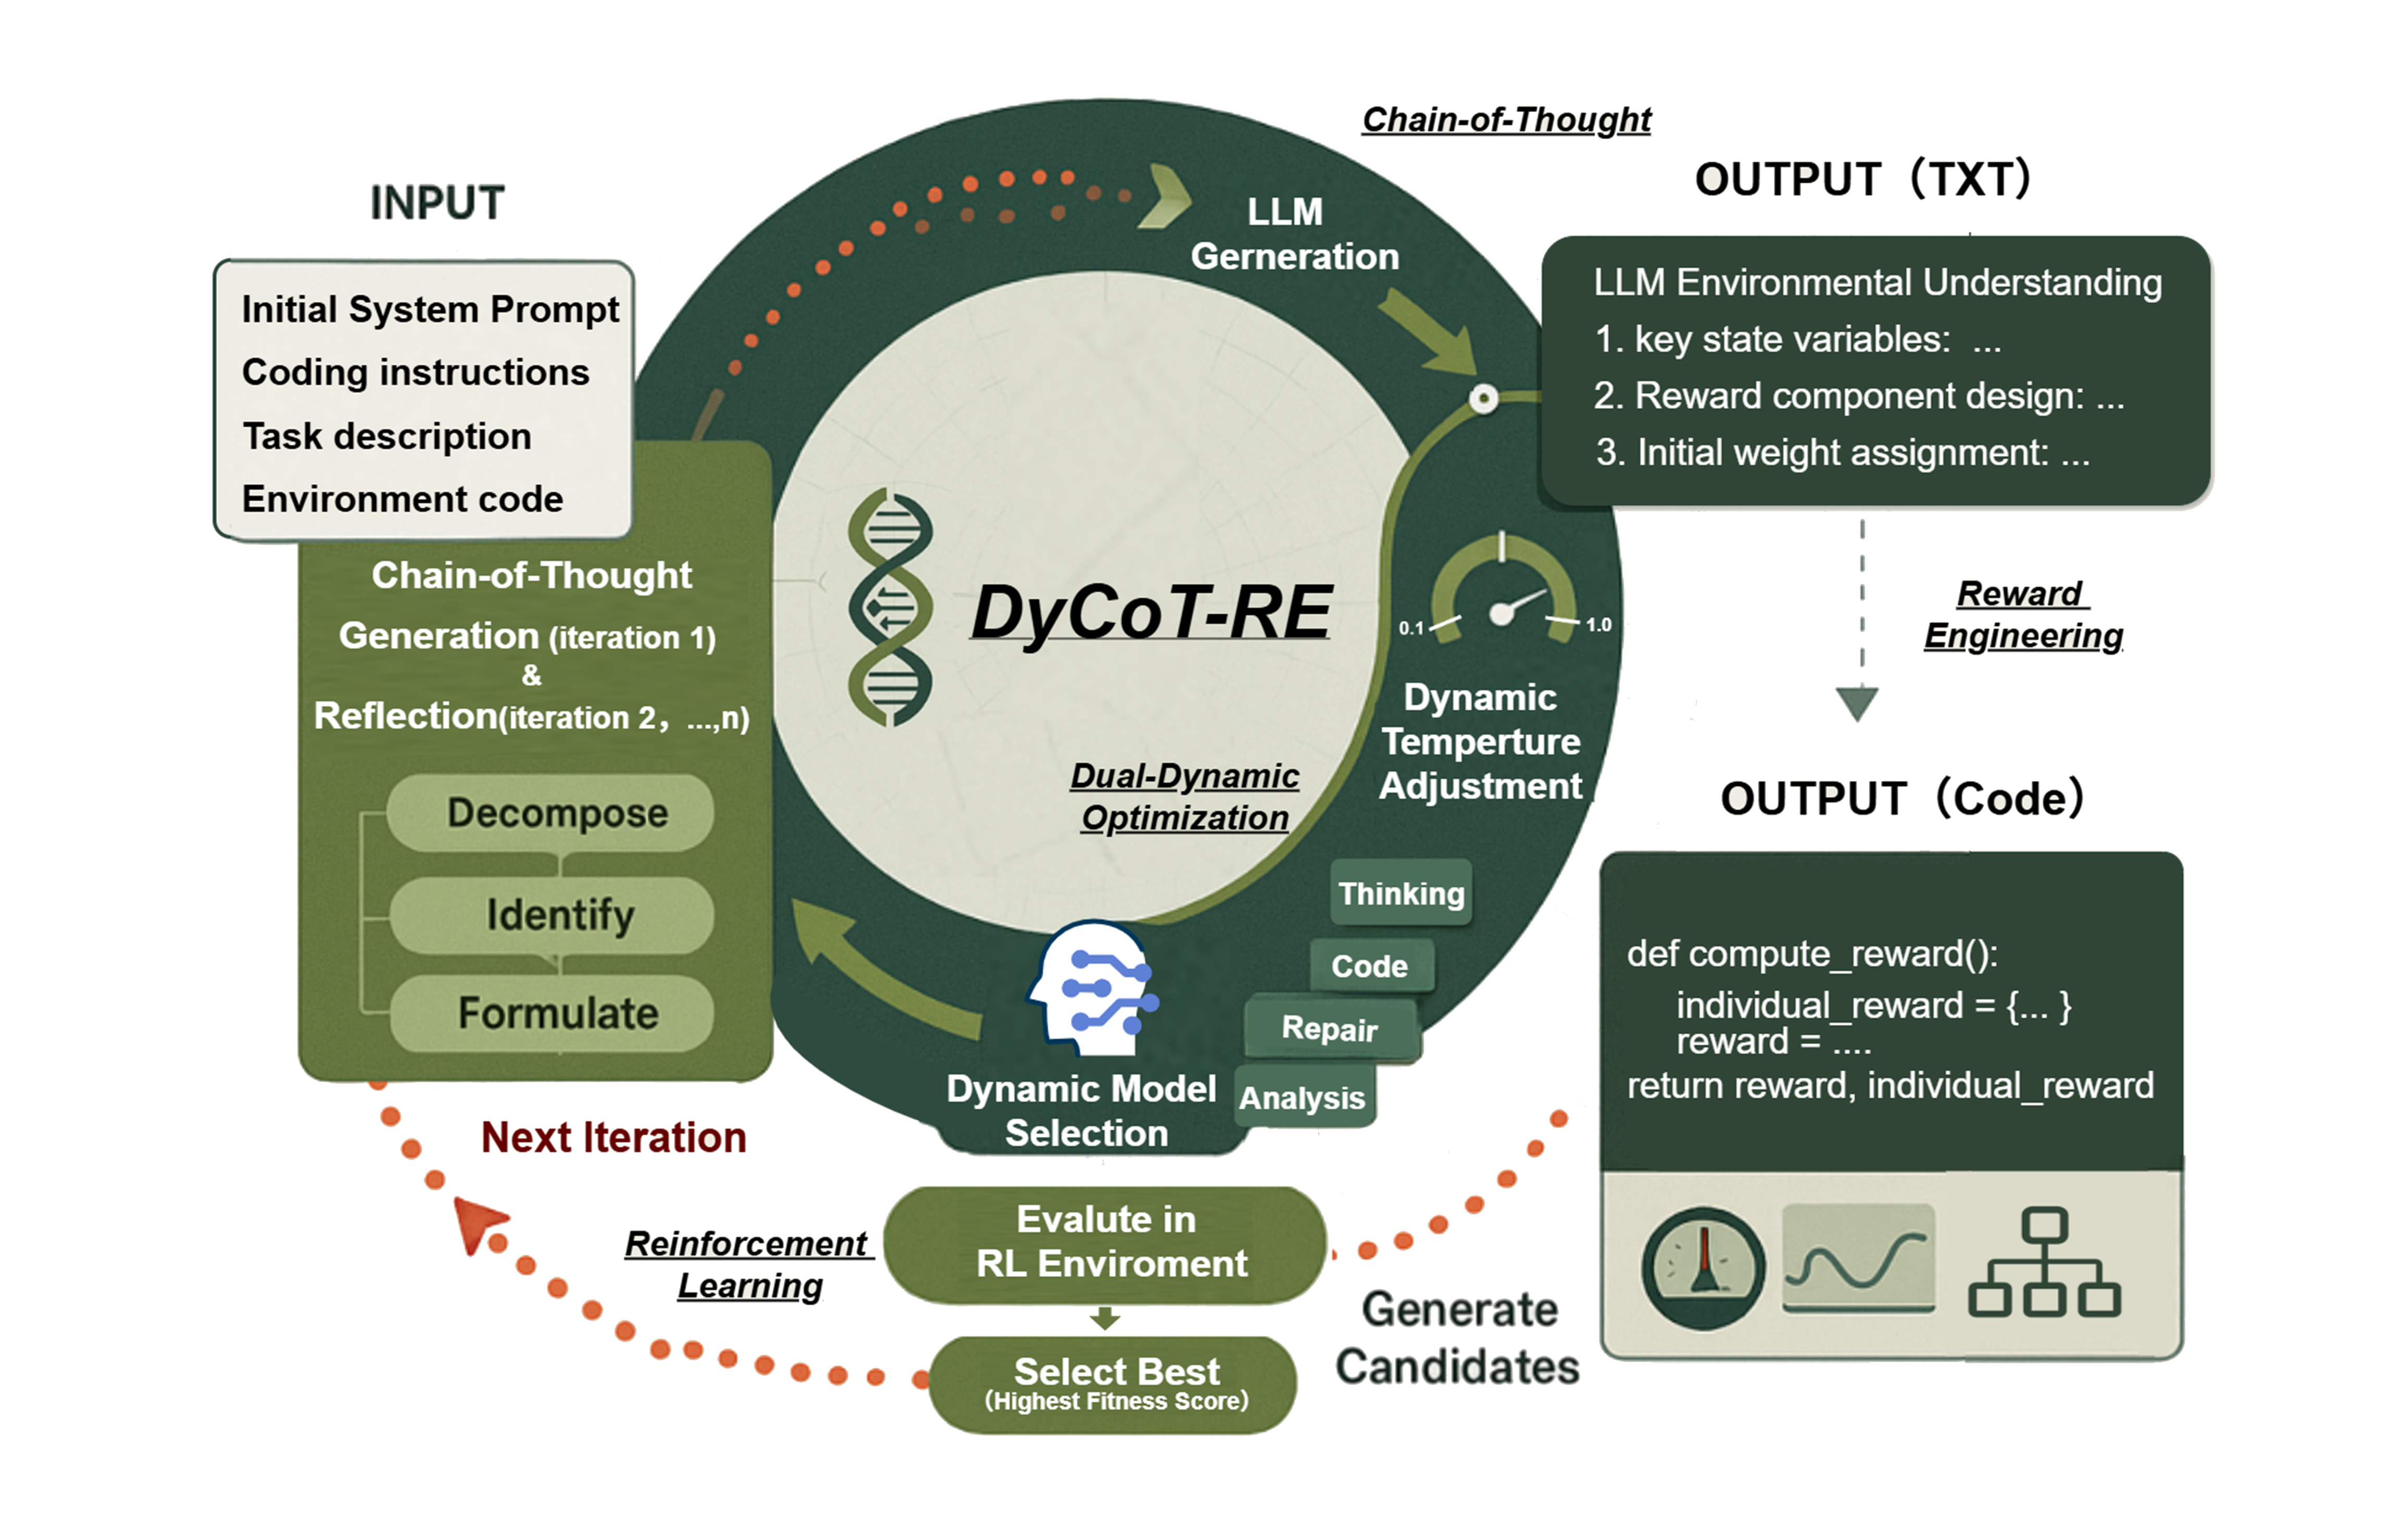
\includegraphics[width=0.85\linewidth]{Figures/dycot-re-architecture.png}
    \caption{DyCoT-RE framework integrating CoT reasoning, dynamic temperature adjustment, and model selection in an evolutionary optimization loop.}
    \label{fig:architecture}
\end{figure*}

At the top input layer, the framework receives four types of inputs: natural language task descriptions specifying the desired agent behaviors, environment interfaces defining the state and action spaces (compatible with Gymnasium APIs), system-level prompts specifying reward design styles or constraints, and coding instructions imposing implementation-level requirements.

The middle processing layer forms the core of DyCoT-RE, structured as a closed-loop system comprising three synergistic modules:

First, the CoT Reasoning Module parses task descriptions into structured subgoals and transforms them into mathematical sub-reward components $r_i(s,a)$ through multi-step semantic decomposition (decompose → identify → formulate). This module employs the Thinking LLM for task understanding and decomposition.

Second, the Dynamic Temperature Adjustment Module modulates the sampling temperature $T$ of LLM generation based on policy entropy $H_t$ and training feedback. As shown in Figure~\ref{fig:control-flow}, it continuously adjusts the exploration–exploitation trade-off, ensuring generative diversity while maintaining stability during reward code synthesis.

Third, the Dynamic Model Selection Module dynamically routes sub-tasks to specialized LLMs, including:
Thinking, Code, Repair and Analysis LLMs. 
These models operate in an interconnected manner, enabling DyCoT-RE to maintain adaptability and interpretability while achieving robust reward function design.

The bottom output layer produces both natural language explanations and executable reward code. The generated reward function

\begin{equation}
R(s,a) = \sum_{i=1}^{m} w_i r_i(s,a)
\end{equation}

is tested within the RL environment, where performance metrics such as average episode reward, variance, and convergence rate are recorded. Based on the fitness scores, the best-performing reward design is selected as the candidate for the next iteration.

Figure~\ref{fig:control-flow} further highlights the evolutionary optimization loop, where:

\begin{equation}
\text{CoT}_{k+1}
=
\text{Analysis}
\circ
\text{Repair}
\circ
\text{Code}
\circ
\text{Thinking}(\text{CoT}_k).
\end{equation}

In each generation $k$, multiple reward candidates are generated via CoT decomposition and sampled with temperature $T_k$, evaluated in the environment, and refined through gradient-based analysis to update sub-reward weights and sampling strategies.

The dual-dynamic optimization, represented as the DNA double helix in Figure~\ref{fig:architecture}, emphasizes the synergistic coupling of temperature modulation (controlling generative stochasticity) and model selection (allocating specialized LLM expertise). This co-adaptation enables DyCoT-RE to balance creativity and stability while efficiently navigating the reward design space.

Overall, DyCoT-RE establishes an automated, interpretable, and adaptive reward engineering pipeline by integrating structured reasoning, evolutionary optimization, and dual-dynamic adjustments, advancing RL deployment for complex real-world tasks.


\subsection{Chain-of-Thought Reasoning for Reward Engineering}

Let $d$ denote the task description and $s,a$ the state-action pair. The reward function is decomposed into:

\begin{equation}
R(s,a) = \sum_{i=1}^{m} w_i \cdot r_i(s,a),
\end{equation}

where $r_i(s,a)$ is the sub-reward for subgoal $i$, generated via CoT parsing:

\begin{equation}
r_i(s,a) = \text{CoT}(I_i),
\end{equation}

with $I_i = \{ \text{subgoal}_i, \text{env\_constraints} \}$. For example, minimizing torso tilt is formulated as:

\begin{equation}
r_1(s,a) = -|\theta_{\text{tilt}}(s)|.
\end{equation}

The initial weights $w_i^{(0)}$ are derived based on subgoal semantic priorities inferred by the LLM, and are refined 
iteratively according to gradient feedback. The policy parameters $\theta$ are updated as:

\begin{equation}
\theta_{t+1} = \theta_t + \alpha \nabla_\theta J(\theta),
\end{equation}

where $J(\theta)$ is the expected cumulative reward:

\begin{equation}
J(\theta) = \mathbb{E}_{\pi_\theta} \left[ \sum_{t=0}^{T} \gamma^t R(s_t,a_t) \right].
\end{equation}

This CoT-based formulation ensures that each sub-reward remains semantically interpretable and traceable to its natural language origin.

\subsection{Dual-Dynamic Optimization Strategy}

Figure~\ref{fig:control-flow} illustrates the coupled feedback architecture of dual-dynamic optimization, which comprises temperature 
adjustment and model selection operating synergistically.

\begin{figure*}[t]
    \centering
    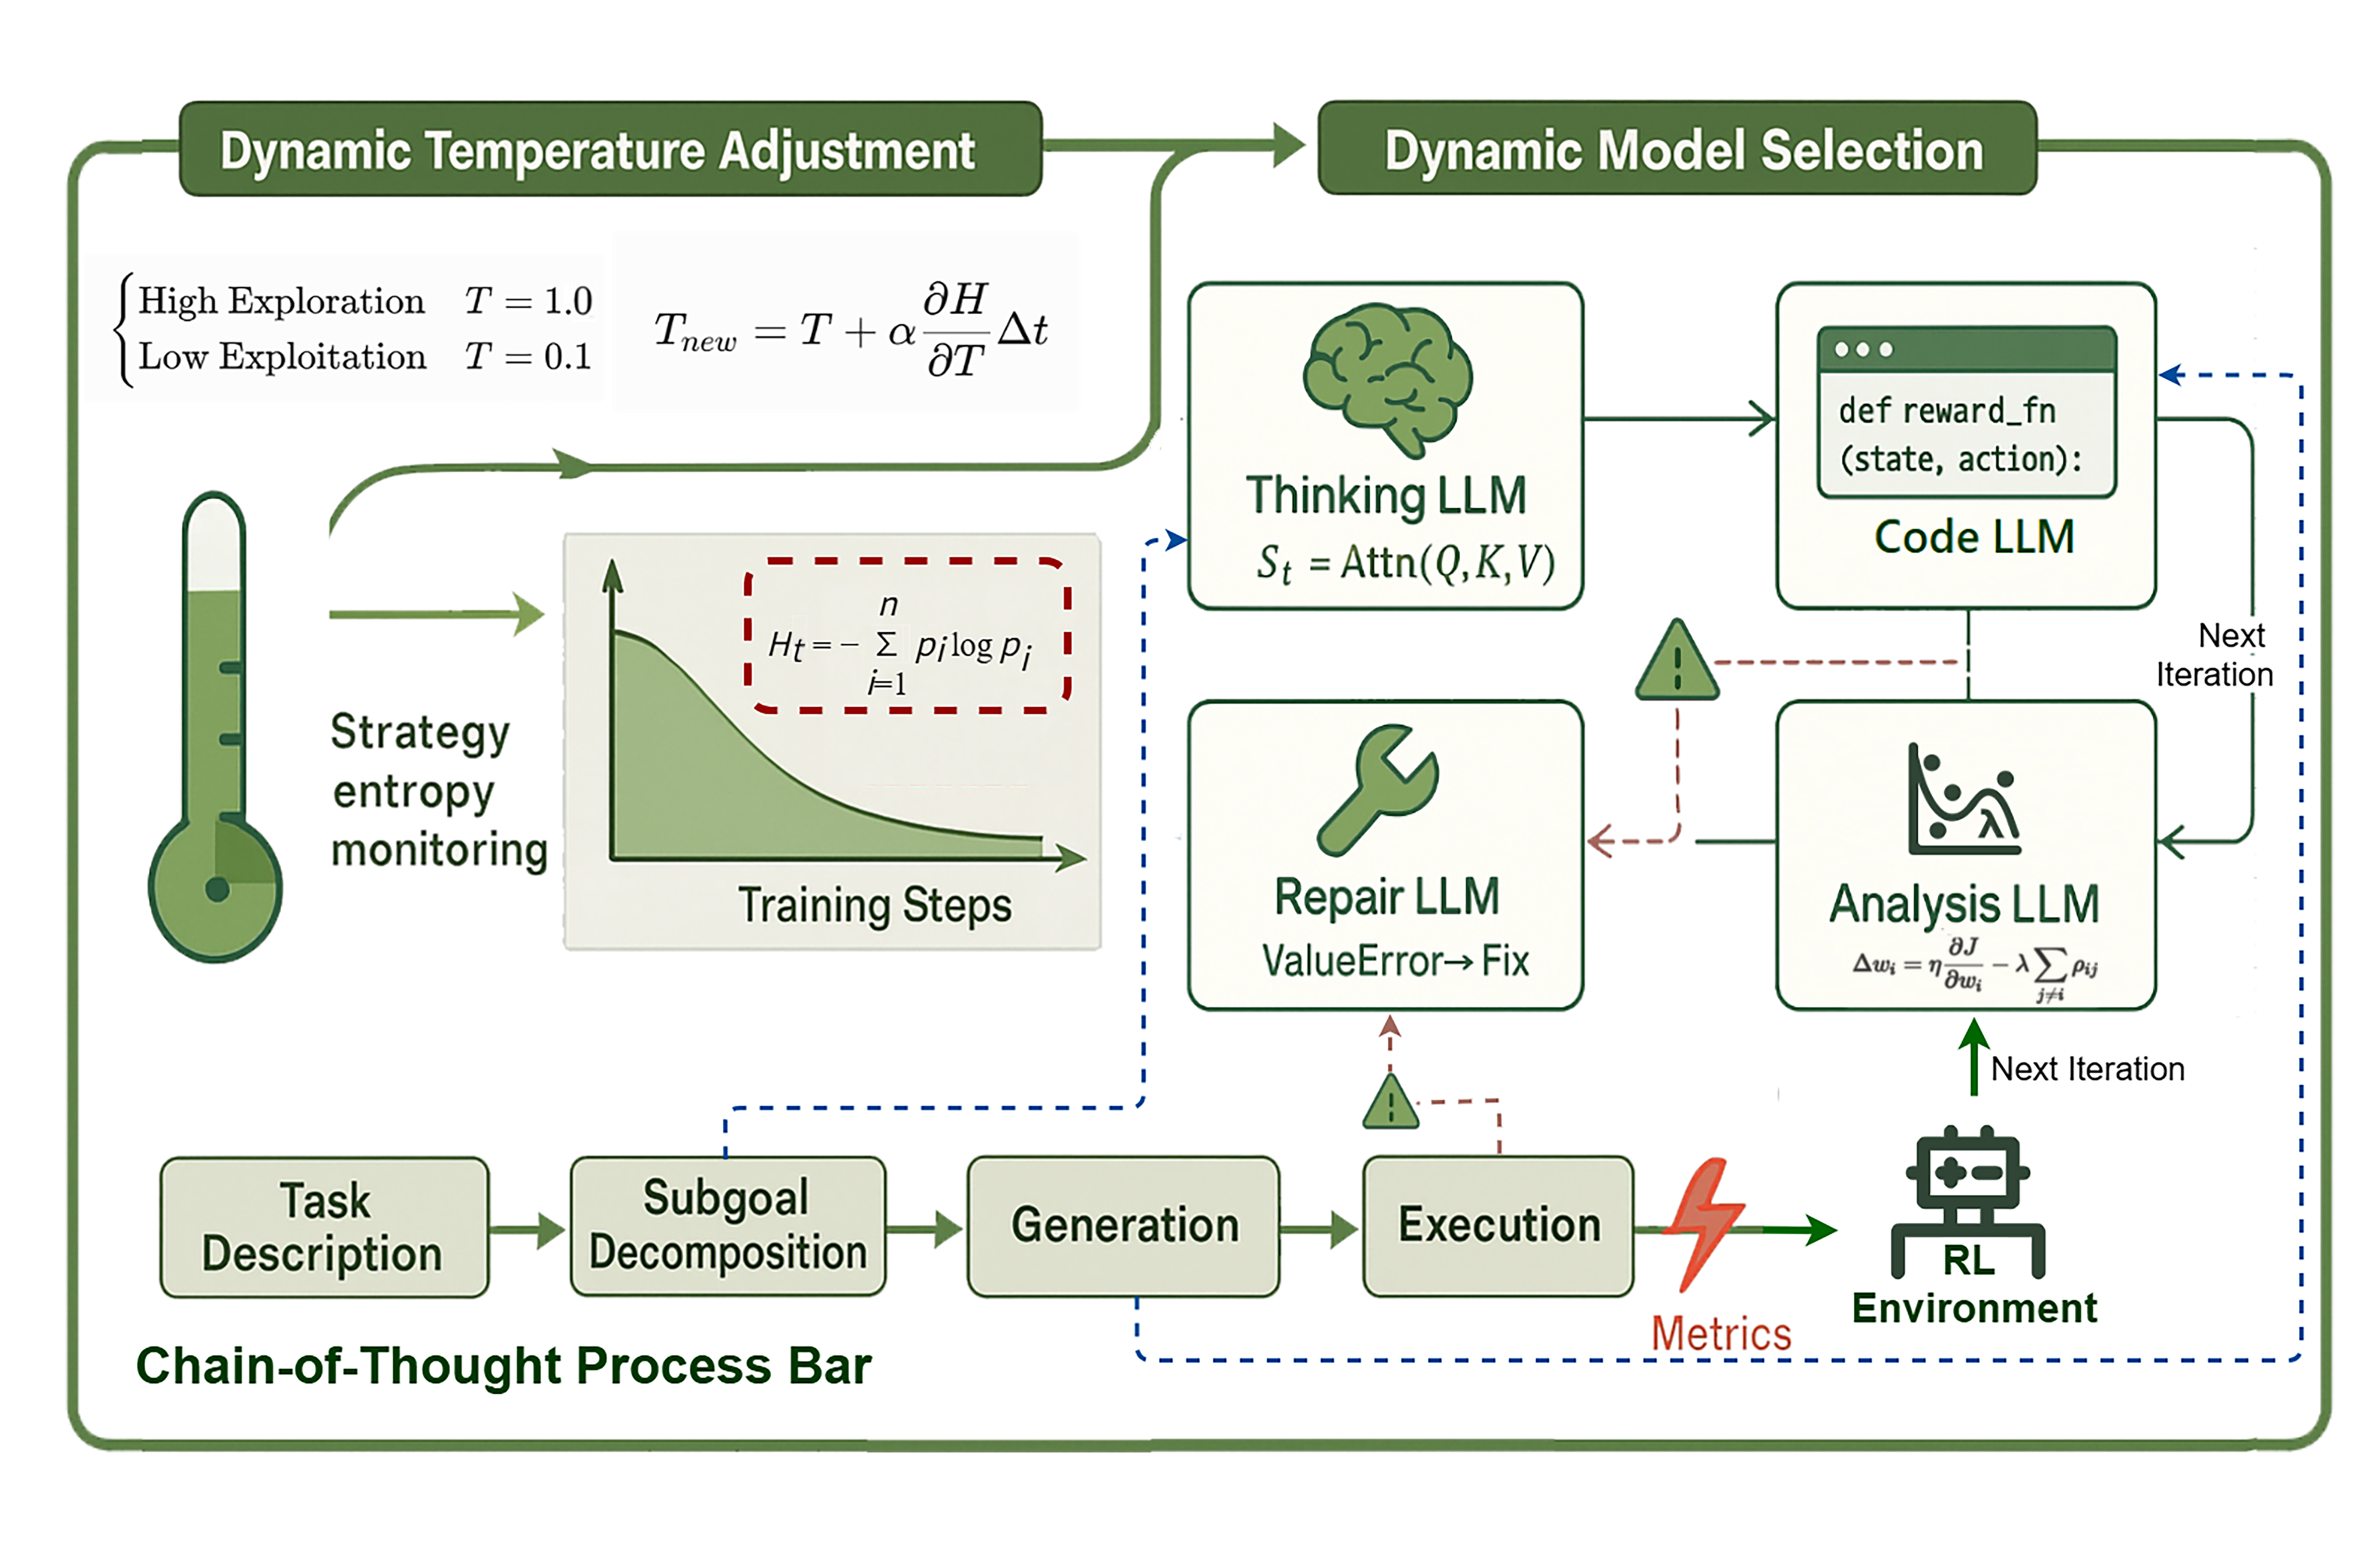
\includegraphics[width=0.85\linewidth]{Figures/dycot-re-control-flow.png}
    \caption{DyCoT-RE dynamic control flow integrating temperature modulation and model selection with CoT iterative reasoning.}
    \label{fig:control-flow}
\end{figure*}

\subsubsection{Dynamic Temperature Adjustment}

Temperature modulation is formalized as a constrained stochastic optimal control problem. Let $T_t$ be the temperature at iteration $t$, 
$H_t$ the policy entropy, and $\Delta T_t$ the temperature adjustment. The entropy is computed as:

\begin{equation}
H_t = - \sum_{i=1}^{n} p_i \log p_i,
\label{eq:entropy}
\end{equation}

where $p_i$ are normalized probabilities over action selections. The temperature update follows:

\begin{equation}
T_{t+1} = T_t + \alpha \frac{\partial T}{\partial H_t} \Delta t,
\label{eq:temp_update}
\end{equation}

with $\alpha$ as the learning rate. The adjustment logic satisfies:

\begin{equation}
T_{t+1} = 
\begin{cases}
T_t + \eta_1 (H_t - H_{target}), & \text{if } H_t > H_{target} \\
T_t - \eta_2 (H_{target} - H_t), & \text{otherwise},
\end{cases}
\end{equation}

(see also Eq.~\eqref{eq:temp_update}).

The optimal control seeks to maximize:

\begin{equation}
\max_{T} \mathbb{E} \left[ \sum_{t=0}^{\tau} \gamma^t R_t \right],
\end{equation}

subject to Lyapunov stability conditions:

\begin{equation}
\dot{V}(T) \leq -\eta V(T), \quad \eta > 0.
\end{equation}


\subsubsection{Dynamic Model Selection}

In DyCoT-RE, dynamic model selection refers to the adaptive routing of different sub-tasks in the reward engineering pipeline to specialized LLMs according to their functional strengths and the current training context.

Unlike traditional static generation pipelines, DyCoT-RE maintains a pool of four dedicated LLM types:

\begin{enumerate}
    \item \textbf{Thinking LLM} ($\mathcal{M}_{\text{think}}$) focuses on semantic parsing, environment understanding, and task decomposition. It processes natural language descriptions to identify structured subgoals and relevant state-action variables for reward formulation, as in Eq.~\eqref{eq:thinkingllm}.
    
    \item \textbf{Code LLM} ($\mathcal{M}_{\text{code}}$) specializes in synthesizing executable reward functions based on decomposed subgoals and prior analysis feedback, as in Eq.~\eqref{eq:reward_agg}.
    
    \item \textbf{Repair LLM} ($\mathcal{M}_{\text{repair}}$) is activated when code execution errors arise during environment evaluation, as in Eq.~\eqref{eq:repairllm}.
    
    \item \textbf{Analysis LLM} ($\mathcal{M}_{\text{analysis}}$) evaluates reward candidate performance, computes gradients for sub-reward weight updates, and recommends adjustments, as in Eq.~\eqref{eq:analysisllm}.
\end{enumerate}

Dynamic model selection within DyCoT-RE governs the allocation of reward engineering sub-tasks to these four specialized LLMs. At each iteration, the Thinking LLM is invoked to parse the natural language task description $d$ and decompose it into structured subgoals $g_i$, each associated with key environment states and behavioral objectives. Mathematically, this semantic parsing can be conceptualized as:

\begin{equation}
g_i = \mathcal{M}_{\text{think}}(d, E),
\label{eq:thinkingllm}
\end{equation}

where $E$ denotes the environment specification.

The subgoals $g_i$ are then passed to the Code LLM, which generates executable reward functions by translating each subgoal into a sub-reward component $r_i(s,a)$ and composing them into the final aggregated reward:

\begin{equation}
R(s,a) = \sum_{i=1}^{m} w_i r_i(s,a),
\label{eq:reward_agg}
\end{equation}

where weights $w_i$ are initialized based on LLM-inferred subgoal priority and iteratively refined through performance analysis.

During execution within the RL environment, if runtime errors occur (e.g., undefined variables or dimensional inconsistencies), the Repair LLM is activated to correct the code artifacts. Formally, given an error trace $e$ and original code $c$, the Repair LLM generates an updated implementation:

\begin{equation}
c' = \mathcal{M}_{\text{repair}}(e, c).
\label{eq:repairllm}
\end{equation}

Post-execution, the Analysis LLM evaluates policy performance by calculating rollout-based metrics such as expected cumulative reward $J(\theta)$ and reward variance $\sigma_R^2$. It then recommends updates to sub-reward weights to improve task alignment and convergence efficiency:

\begin{equation}
w_i^{(t+1)} = w_i^{(t)} + \eta \frac{\partial J(\theta)}{\partial w_i} - \lambda \sum_{j \neq i} \rho_{ij},
\label{eq:analysisllm}
\end{equation}

where $\rho_{ij}$ represents the Pearson correlation coefficient between sub-reward components to penalize redundancy, and $\eta, \lambda$ are learning rate and regularization hyperparameters, respectively.

Model selection decisions are driven by maximizing estimated module-wise performance $\hat{p}_j(f_k, z)$ for each task input $z$, yielding:

\begin{equation}
k_j^* = \arg\max_{k \in M} \hat{p}_j(f_k, z),
\end{equation}

where $k_j^*$ is the optimal model choice for module $j$ from candidate set $M$.

Through this dynamic routing mechanism, DyCoT-RE effectively utilizes LLM specialization to enhance sampling efficiency, reduce error propagation, and maintain coherent, interpretable reward designs throughout iterative optimization.


\subsubsection{Joint Adaptive Optimization}

The dual-dynamic optimization strategy in DyCoT-RE integrates temperature adjustment and model selection into a closed-loop, mutually adaptive system to enhance reward function quality and training efficiency. Unlike independent application of these mechanisms, their joint operation forms a synergistic optimization pathway aligning language model sampling dynamics with reinforcement learning objectives.

At each iteration $t$, the Thinking LLM decomposes the task description into structured subgoals, producing an initial reward design $R_t(s,a)$. This design is passed to the Code LLM to generate executable Python code for environment evaluation. During agent training with policy $\pi_{\theta}$, the policy entropy $H_t$ is computed as:

\begin{equation}
H_t = - \sum_{a \in \mathcal{A}} \pi_{\theta}(a|s_t) \log \pi_{\theta}(a|s_t),
\end{equation}

quantifying exploration stochasticity. Simultaneously, rollout-based performance metrics, including expected return $J(\theta)$ and reward variance $\sigma_R^2$, are monitored:

\begin{equation}
J(\theta) = \mathbb{E}_{\pi_\theta} \left[ \sum_{k=0}^{T} \gamma^k R(s_k,a_k) \right],
\end{equation}
\begin{equation}
\sigma_R^2 = \mathbb{E}[(R - \mathbb{E}[R])^2].
\end{equation}

The Dynamic Temperature Adjustment module uses these feedback signals to update the sampling temperature $T$ according to:

\begin{equation}
T_{t+1} = T_t + \alpha \left( \frac{\partial T}{\partial H_t} \Delta t \right),
\end{equation}

where $\alpha$ is the learning rate controlling update smoothness, and $\frac{\partial T}{\partial H_t}$ represents sensitivity of temperature to entropy deviation from the target. Higher policy entropy relative to the target increases $T$, promoting more diverse LLM generations to facilitate exploration, while lower entropy triggers a temperature decrease to stabilize sampling outputs.

Concurrently, the Dynamic Model Selection module evaluates module-wise performance of candidate LLMs based on local quality estimations $\hat{p}_j(f_k, z)$ and global training improvements:

\begin{equation}
k_j^* = \arg\max_{k \in M} \left[ \hat{p}_j(f_k, z) + \gamma \cdot J(\theta) \right],
\end{equation}

where $\gamma$ controls the influence of global reward performance on model routing decisions.

Critically, these two dynamic adjustments interact adaptively. Temperature adjustment influences the sampling diversity of the Code LLM, affecting candidate reward variants’ distribution and consequently altering the inputs for model selection. Conversely, model selection decisions affect the generation quality and robustness of reward functions, which modulate agent behavior, impacting policy entropy and subsequent temperature updates.

This mutual adaptation forms a coupled optimization system expressed abstractly as:

\begin{equation}
\begin{cases}
T_{t+1} = f_T(H_t, J(\theta), \sigma_R^2), \\
k_j^* = g_k(T_t, \hat{p}_j(f_k, z), J(\theta)),
\end{cases}
\end{equation}

where $f_T$ and $g_k$ denote the temperature update and model selection policies, respectively.

To ensure convergence and stability, a Lyapunov-based condition is enforced:

\begin{equation}
\frac{\partial^2 T}{\partial H^2}
+ \frac{\partial^2 T}{\partial C^2}
\leq \frac{2}{\eta} \left( \frac{\partial R}{\partial T} \right)^2,
\end{equation}

with $\eta$ representing a Lipschitz constant bounding system gradients. This guarantees that the joint temperature-model adjustment does not induce oscillatory divergence during training.

Overall, this integrated dual-dynamic optimization framework enables DyCoT-RE to adaptively balance exploration and exploitation while efficiently leveraging specialized LLM capabilities for interpretable reward function generation across diverse RL tasks.

\section{Experiments}


\subsection{Experimental Setup}

\subsubsection{Environments}

We evaluate DyCoT-RE on four reinforcement learning environments that span diverse task structures and complexities. 
The standard benchmarks include CartPole (discrete pole balancing), BipedalWalker (continuous biped locomotion), 
and Ant (high-dimensional quadruped control). 
Additionally, we design a custom SpaceMining environment to assess generalization to novel multi-agent resource collection 
tasks beyond standard benchmarks. All environments are implemented using the Gymnasium platform. 
For baseline comparisons, official Gymnasium reward functions are used in standard tasks, 
while SpaceMining employs a manually designed heuristic reward emphasizing resource efficiency and collision avoidance.

\subsubsection{Baselines}

We evaluate DyCoT-RE against two representative baselines to contextualize its performance:

\textbf{(1) Human-designed rewards}  
Standard expert-crafted reward functions using Gymnasium's native implementations for CartPole, BipedalWalker, and Ant, 
with manual heuristics for SpaceMining. This reflects the traditional gold standard in RL.

\textbf{(2) Eureka}  
A pioneering LLM-based framework that demonstrated LLMs' potential in automated reward design through code synthesis and verification. 
As a foundational work in this space, it provides a natural reference for assessing our incremental improvements. 
While Eureka focuses on direct code generation without CoT or dynamic optimization, we adapt its pipeline to our Gymnasium-based 
evaluation settings for consistency.

Additionally, to assess the contribution of each DyCoT-RE module, Section~\ref{sec:ablation} conducts ablation studies 
comparing DyCoT-RE against its internal variants:

- Zero-shot reward generation without CoT reasoning

- DyCoT-RE without temperature adjustment

- DyCoT-RE without model selection

Due to computational constraints and consistent observed trends across environments, 
temperature adjustment and model selection ablation were conducted on BipedalWalker as a representative continuous control task, 
while CoT reasoning was evaluated on all four environments to confirm its general effectiveness.


\subsubsection{Implementation Details}

All experiments use PPO from Stable-Baselines3, with hyperparameters summarized in Table~\ref{tab:env_settings}. 
Policy networks employ two-layer MLPs ([64,64] units) for single-agent tasks and a larger [256,256,128] MLP for SpaceMining. 
Models are trained with Adam (learning rate 0.0003), batch size 64, GAE $\lambda=0.95$, and 
discount factor $\gamma=0.999$ ($0.99$ for SpaceMining).

Reward generation uses DyCoT-RE with a local LLM backend deployed via Ollama. 
Each CoT iteration produces 8 candidate rewards in parallel at a temperature of 0.6, enabling controlled diversity. 
No handcrafted prompt templates are used to promote open-ended generation. 
Final evaluations report mean performance over 10 test episodes with varied seeds. 
GPU resource management automatically releases memory when utilization exceeds 60\%, ensuring stable parallel execution.

\begin{table}[ht]
\centering
\caption{Environment-specific experimental settings.}
\label{tab:env_settings}
\begin{tabular}{lcccc}
\hline
Environment & Max Steps & Total Steps & Parallel Env & CoT Iter\\
\hline
CartPole-v1 & 500 & $10^4$ & 4 & 5 \\
BipedalWalker-v3 & 1600 & $10^6$ & 10 & 8 \\
Ant-v5 & 1600 & $5 \times 10^6$ & 10 & 8 \\
SpaceMining & 1600 & $3 \times 10^6$ & 8 & 8 \\
\hline
\end{tabular}
\end{table}



\subsection{Overall Performance}


This section summarizes the performance of DyCoT-RE compared to baselines across four representative reinforcement learning environments.


\begin{figure*}[t]
\centering
\includegraphics[width=0.85\linewidth]{Figures/reward_episode_curve.png}
\caption{Learning curves of DyCoT-RE (blue) vs Human-designed rewards (green) across training timesteps.}
\label{fig:learning_curves}
\end{figure*}

Figure~\ref{fig:learning_curves} shows that in CartPole, a simple discrete control task with dense and informative rewards, 
DyCoT-RE achieves slightly faster convergence than the Human-designed baseline, but the final reward difference remains small. 
This is expected, as the environment’s inherent simplicity and clear feedback signals allow even heuristic rewards to perform well, 
limiting the potential benefit from additional reward optimization.

In other environments, the advantages of DyCoT-RE are more apparent. For example, in BipedalWalker, which requires coordinated control 
of multiple joints under sparse and noisy feedback, DyCoT-RE produces smoother learning curves and achieves higher final rewards. 
Its structured reward decomposition may help the agent acquire stable walking gaits by explicitly separating balance and propulsion objectives.

In Ant, a high-dimensional locomotion task, both methods initially experience unstable exploration with reward drops. 
However, DyCoT-RE recovers earlier—around 1.2 million timesteps—and continues improving towards higher rewards. 
This suggests that DyCoT-RE is better able to resolve credit assignment challenges in redundant action spaces, accelerating policy learning in later training stages.

In the SpaceMining environment, designed to test generalization to novel resource collection tasks, DyCoT-RE maintains a steadily increasing learning curve 
and achieves final rewards close to 2000, while Human-designed rewards remain relatively flat. 
This indicates that DyCoT-RE’s adaptive reward generation can extract useful signals even in tasks lacking predefined heuristic reward functions.

\begin{figure}[t]
\centering
\includegraphics[width=0.48\textwidth]{Figures/bar_comparison_3.png}
\caption{Final average rewards across environments comparing Human-designed, Eureka, and DyCoT-RE.}
\label{fig:bar_comparison}
\end{figure}

Figure~\ref{fig:bar_comparison} compares final average rewards across methods. 
DyCoT-RE achieves noticeably higher rewards in Cartpole, BipedalWalker, Ant, and SpaceMining. 
These results demonstrate that the integration of Chain-of-Thought reasoning with dynamic optimization in DyCoT-RE provides meaningful 
benefits, particularly in environments with sparse feedback or complex task structures.


\subsection{Ablation Study}
\label{sec:ablation}

This section conducts an ablation study to examine the individual contribution of each component in DyCoT-RE, including CoT reasoning, temperature adjustment, and model selection, as well as their combined synergistic effects.

\subsubsection{Impact of CoT Reasoning}


We evaluate the impact of incorporating Chain-of-Thought (CoT) reasoning into reward engineering by comparing DyCoT-RE's CoT-enabled variant against a zero-shot baseline lacking structured intermediate reasoning.


\begin{figure}[t]
\centering
\includegraphics[width=0.48\textwidth]{Figures/cot_ablation.png}
\caption{Final reward distributions for CoT-enabled vs zero-shot reward generation across environments.}
\label{fig:cot_ablation}
\end{figure}


Figure~\ref{fig:cot_ablation} summarizes reward distributions for both methods across the four benchmark environments. A consistent pattern emerges: CoT-enabled rewards exhibit higher means, lower variance, and reduced outlier incidence compared to zero-shot. In CartPole and SpaceMining, CoT-enabled results are tightly clustered near the environment's upper performance bounds, whereas zero-shot results are widely dispersed, with a substantial proportion of runs yielding suboptimal or even near-zero rewards. This reflects CoT's ability to systematically decompose task objectives into interpretable sub-rewards, enhancing sample efficiency and stabilizing policy learning.


In BipedalWalker, an illustrative deviation is observed. While CoT-enabled runs achieve rewards concentrated between 250–310 with minimal negative outcomes, zero-shot results present a bimodal distribution: one cluster achieves moderate positive rewards ($\sim$150–250), while another cluster yields severely negative rewards (e.g. -124, -97, -73). This bimodality indicates that without structured reasoning, reward generation often fails to encode essential balance or locomotion constraints, resulting in policies that collapse during gait training.


Taken together, these results illustrate that CoT reasoning reliably improves reward interpretability and training stability, especially in settings with sparse or ambiguous feedback.



\subsubsection{Impact of Temperature Adjustment}

Next, we investigate the effect of temperature settings by sweeping $T \in [0.0, 1.0]$ on the BipedalWalker environment. 
Table~\ref{tab:temp_sweep} summarizes the results, including average fitness, maximum/minimum fitness, standard deviation, and reward efficiency ratio (average fitness divided by standard deviation).

\begin{table}[ht]
\centering
\caption{BipedalWalker performance under different temperature settings. Top-1 temperature is highlighted in green, DyCoT-RE result in blue.}
\label{tab:temp_sweep}
\begin{tabular}{c|c|c|c|c}
\hline
Temp & Avg Fit$\uparrow$ & Max/Min Fit $\uparrow$& Std$\downarrow$  & Eff. Ratio$\uparrow$ \\
\hline
0.0 & 81.93 & 301.15/-53.01 & 148.67 & 0.55 \\
0.1 & 149.56 & 310.94/-33.73 & 155.22 & 0.96 \\
0.2 & 242.74 & 313.60/-20.27 & 125.47 & 1.93 \\
0.3 & 210.07 & 311.17/-46.69 & 140.49 & 1.50 \\
\rowcolor{green!15}
0.4 & 244.19 & 311.94/-17.13 & 107.02 & 2.28 \\
0.5 & 215.84 & 310.69/-14.25 & 131.01 & 1.65 \\
\rowcolor{green!25}
0.6 & 248.11 & 312.48/-21.18 & 120.45 & 2.06 \\
0.7 & 225.88 & 312.42/-12.08 & 131.43 & 1.72 \\
0.8 & 74.33 & 310.42/-46.72 & 143.91 & 0.52 \\
0.9 & 145.02 & 310.02/-31.58 & 148.51 & 0.98 \\
1.0 & 192.38 & 310.40/-39.05 & 138.37 & 1.39 \\
\rowcolor{blue!15}
DyCoT-RE & \textbf{292.8} & 315.6/87.2 & 55.2 & 5.30 \\
\hline
\end{tabular}
\end{table}

Static sweeps show that mid-range temperatures ($T=0.4$–$0.6$) yield higher fitness and lower variance than extremes. 
DyCoT-RE’s dynamic temperature regulation consistently outperforms these static settings, 
adapting temperature during training to maintain an effective exploration-exploitation trade-off. 


\subsubsection{Impact of Model Selection}

Finally, we evaluate the impact of DyCoT-RE's dynamic model selection by comparing it against individual static LLM baselines on the BipedalWalker environment. Table~\ref{tab:model_selection} summarizes average fitness, max/min fitness, standard deviation, and reward efficiency ratio (average fitness divided by standard deviation). Only models with sufficient sample sizes ($N>10$) are included.

DyCoT-RE achieves the highest average fitness (\cellcolor{blue!15}307.28) with exceptionally low standard deviation (\cellcolor{blue!15}6.00) and the best efficiency ratio (\cellcolor{blue!15}51.21), demonstrating its capability to consistently generate high-quality rewards across diverse sub-tasks. 

In contrast, while \texttt{codegemma} achieves competitive performance (Avg Fit: 260.8), its higher standard deviation (115.2) results in a substantially lower efficiency ratio (2.26), indicating reduced stability and generalizability compared to DyCoT-RE.

\begin{table*}[ht]
\centering
\caption{Performance comparison of different LLM backends (N=20) in BipedalWalker. $\uparrow$: higher is better; $\downarrow$: lower is better. Green: per-column best baseline. Blue: DyCoT-RE (dynamic selection).}
\label{tab:model_selection}
\begin{tabular}{l|c|c|c|c|c}
\hline
Model (size) & Avg Fit $\uparrow$ & Max Fit $\uparrow$ & Min Fit $\uparrow$ & Std $\downarrow$ & Eff. Ratio $\uparrow$ \\
\hline
codegemma (7b) & 260.8 & 301.8 & \cellcolor{green!25}34.2 & \cellcolor{green!25}75.2 & 3.46\cellcolor{green!25} \\
codeqwen (7b) & 32.6 & 307.6 & -76.0 & 98.4 & 0.33 \\
deepseek-coder (6.7b) & -4.5 & 295.3 & -98.2 & 94.1 & -0.05 \\
deepseek-r1 (8b) & 44.6 & \cellcolor{green!25}321.2 & -99.6 & 122.1 & 0.37 \\
gemma3 (4b) & \cellcolor{green!25}278.0 & 314.8 & -34.2 & 82.0 & 3.39 \\
llama3.1 (8b) & 162.2 & 318.4 & -80.4 & 150.8 & 1.08 \\
qwen2.5 (7b) & 177.0 & 319.5 & -97.2 & 151.5 & 1.17 \\
qwen2.5-coder (7b) & 125.6 & 313.7 & -70.8 & 163.2 & 0.77 \\
\rowcolor{blue!15}
DyCoT-RE & \textbf{297.28} & \textbf{316.57} & \textbf{89.47} & \textbf{46.00} & \textbf{6.46} \\
\hline
\end{tabular}
\end{table*}

While individual models occasionally excel on narrow tasks, DyCoT-RE’s dynamic model routing provides the most generalizable performance, 
effectively balancing reward quality, stability, and adaptability in complex continuous control environments.

In summary, the ablation study demonstrates that each module—CoT reasoning, temperature adjustment, and model selection—contributes significantly to DyCoT-RE’s superior performance, and their combination leads to synergistic gains.



\section{Discussion}
Our comprehensive evaluation of DyCoT-RE across multiple environments and comparison baselines reveals several fundamental insights about reward design in reinforcement learning. The experimental results collectively demonstrate that DyCoT-RE represents a significant advancement in addressing the core challenges of reward engineering, particularly in complex, high-dimensional environments.

The performance advantages observed across all test environments (CartPole, BipedalWalker, Ant, and SpaceMining) underscore the robustness of our approach. Particularly noteworthy is DyCoT-RE's consistent outperformance in the most complex environments (Ant and SpaceMining), where traditional human-designed rewards and simpler baseline methods struggle to achieve comparable results. This suggests that our framework's combination of structured reasoning, dynamic adaptation, and model diversity provides unique advantages for solving challenging control problems that require sophisticated policy learning.

The ablation studies provide critical insights into the individual contributions of each component. The CoT reasoning module proved essential for handling complex reward structures, particularly in environments requiring multi-step decision making. The temperature adjustment mechanism demonstrated its value in balancing exploration and exploitation, while the dynamic model selection showed clear benefits in adapting to different reward design requirements. Most importantly, the synergistic interaction between these components produced performance gains that exceeded simple additive effects, confirming the value of our integrated approach.

Comparisons with baseline methods yielded several important findings. The human-designed rewards, while effective in simple environments, showed clear limitations as task complexity increased. This reinforces the well-known challenge of manually engineering rewards for complex control problems. The Eureka baseline, while representing an advanced LLM-based approach, demonstrated the limitations of purely generative methods without structured reasoning or dynamic adaptation. DyCoT-RE's consistent superiority across all environments highlights the necessity of combining multiple advanced techniques for effective reward design.

The visualization results provide additional confirmation of these findings. The clear separation between DyCoT-RE and baseline methods in the scatter plots (Figure~\ref{fig:cot_ablation}) illustrates the quality and stability advantages of our approach. The temperature sweep results (Table~\ref{tab:temp_sweep} and Figure~\ref{fig:temp_lineplot}) show how dynamic adjustment leads to more reliable performance, while the model comparison (Table~\ref{tab:model_perf} and Figure~\ref{fig:model_bar}) demonstrates the benefits of architectural diversity.

From a broader perspective, our work contributes to the growing body of research on AI-assisted reward design. The success of DyCoT-RE suggests that combining modern LLM capabilities with reinforcement learning insights can overcome many of the traditional limitations of reward engineering. Particularly promising is our framework's ability to automatically adapt to different task requirements, as evidenced by its consistent performance across diverse environments.

However, several challenges remain. The computational overhead of dynamic components, while justified by the performance gains, may limit scalability to extremely large-scale problems. Additionally, while DyCoT-RE performs well on the tested environments, its generalization to completely novel task domains remains to be verified. Future work should explore these aspects while also investigating potential synergies with other emerging techniques in reinforcement learning and AI-assisted programming.

In conclusion, DyCoT-RE represents a significant step forward in reward design methodology. By integrating structured reasoning, dynamic adaptation, and model diversity, our framework provides a robust solution to the enduring challenge of effective reward engineering in reinforcement learning. The consistent performance improvements across all test environments, particularly the most complex ones, demonstrate the practical value of our approach and suggest promising directions for future research in this area.

\section{Conclusion}
We propose a dual-dynamic optimization framework for CoT-based RL reward generation, incorporating temperature regulation and model selection. Our results demonstrate improved convergence, stability, and reward quality across tasks, laying a foundation for scalable, self-adaptive reward engineering.

\bibliographystyle{IEEEtran} % 或其他你需要的样式
\bibliography{adaptive_cot_reward_rl} % 不需要加.bib扩展名

\end{document}
